% Template for PLoS
% Version 3.5 March 2018
%
% % % % % % % % % % % % % % % % % % % % % %
%
% -- IMPORTANT NOTE
%
% This template contains comments intended
% to minimize problems and delays during our production
% process. Please follow the template instructions
% whenever possible.
%
% % % % % % % % % % % % % % % % % % % % % % %
%
% Once your paper is accepted for publication,
% PLEASE REMOVE ALL TRACKED CHANGES in this file
% and leave only the final text of your manuscript.
% PLOS recommends the use of latexdiff to track changes during review, as this will help to maintain a clean tex file.
% Visit https://www.ctan.org/pkg/latexdiff?lang=en for info or contact us at latex@plos.org.
%
%
% There are no restrictions on package use within the LaTeX files except that
% no packages listed in the template may be deleted.
%
% Please do not include colors or graphics in the text.
%
% The manuscript LaTeX source should be contained within a single file (do not use \input, \externaldocument, or similar commands).
%
% % % % % % % % % % % % % % % % % % % % % % %
%
% -- FIGURES AND TABLES
%
% Please include tables/figure captions directly after the paragraph where they are first cited in the text.
%
% DO NOT INCLUDE GRAPHICS IN YOUR MANUSCRIPT
% - Figures should be uploaded separately from your manuscript file.
% - Figures generated using LaTeX should be extracted and removed from the PDF before submission.
% - Figures containing multiple panels/subfigures must be combined into one image file before submission.
% For figure citations, please use "Fig" instead of "Figure".
% See http://journals.plos.org/plosone/s/figures for PLOS figure guidelines.
%
% Tables should be cell-based and may not contain:
% - spacing/line breaks within cells to alter layout or alignment
% - do not nest tabular environments (no tabular environments within tabular environments)
% - no graphics or colored text (cell background color/shading OK)
% See http://journals.plos.org/plosone/s/tables for table guidelines.
%
% For tables that exceed the width of the text column, use the adjustwidth environment as illustrated in the example table in text below.
%
% % % % % % % % % % % % % % % % % % % % % % % %
%
% -- EQUATIONS, MATH SYMBOLS, SUBSCRIPTS, AND SUPERSCRIPTS
%
% IMPORTANT
% Below are a few tips to help format your equations and other special characters according to our specifications. For more tips to help reduce the possibility of formatting errors during conversion, please see our LaTeX guidelines at http://journals.plos.org/plosone/s/latex
%
% For inline equations, please be sure to include all portions of an equation in the math environment.
%
% Do not include text that is not math in the math environment.
%
% Please add line breaks to long display equations when possible in order to fit size of the column.
%
% For inline equations, please do not include punctuation (commas, etc) within the math environment unless this is part of the equation.
%
% When adding superscript or subscripts outside of brackets/braces, please group using {}.
%
% Do not use \cal for caligraphic font.  Instead, use \mathcal{}
%
% % % % % % % % % % % % % % % % % % % % % % % %
%
% Please contact latex@plos.org with any questions.
%
% % % % % % % % % % % % % % % % % % % % % % % %

\documentclass[10pt,letterpaper]{article}
\usepackage[top=0.85in,left=2.75in,footskip=0.75in]{geometry}

% amsmath and amssymb packages, useful for mathematical formulas and symbols
\usepackage{amsmath,amssymb}

% Use adjustwidth environment to exceed column width (see example table in text)
\usepackage{changepage}

% Use Unicode characters when possible
\usepackage[utf8x]{inputenc}

% textcomp package and marvosym package for additional characters
\usepackage{textcomp,marvosym}

% cite package, to clean up citations in the main text. Do not remove.
% \usepackage{cite}

% Use nameref to cite supporting information files (see Supporting Information section for more info)
\usepackage{nameref,hyperref}

% line numbers
\usepackage[right]{lineno}

% ligatures disabled
\usepackage{microtype}
\DisableLigatures[f]{encoding = *, family = * }

% color can be used to apply background shading to table cells only
\usepackage[table]{xcolor}

% array package and thick rules for tables
\usepackage{array}

% create "+" rule type for thick vertical lines
\newcolumntype{+}{!{\vrule width 2pt}}

% create \thickcline for thick horizontal lines of variable length
\newlength\savedwidth
\newcommand\thickcline[1]{%
  \noalign{\global\savedwidth\arrayrulewidth\global\arrayrulewidth 2pt}%
  \cline{#1}%
  \noalign{\vskip\arrayrulewidth}%
  \noalign{\global\arrayrulewidth\savedwidth}%
}

% \thickhline command for thick horizontal lines that span the table
\newcommand\thickhline{\noalign{\global\savedwidth\arrayrulewidth\global\arrayrulewidth 2pt}%
\hline
\noalign{\global\arrayrulewidth\savedwidth}}


% Remove comment for double spacing
%\usepackage{setspace}
%\doublespacing

% Text layout
\raggedright
\setlength{\parindent}{0.5cm}
\textwidth 5.25in
\textheight 8.75in

% Bold the 'Figure #' in the caption and separate it from the title/caption with a period
% Captions will be left justified
\usepackage[aboveskip=1pt,labelfont=bf,labelsep=period,justification=raggedright,singlelinecheck=off]{caption}
\renewcommand{\figurename}{Fig}

% Use the PLoS provided BiBTeX style
% \bibliographystyle{plos2015}

% Remove brackets from numbering in List of References
\makeatletter
\renewcommand{\@biblabel}[1]{\quad#1.}
\makeatother



% Header and Footer with logo
\usepackage{lastpage,fancyhdr,graphicx}
\usepackage{epstopdf}
%\pagestyle{myheadings}
\pagestyle{fancy}
\fancyhf{}
%\setlength{\headheight}{27.023pt}
%\lhead{
\includegraphics[width=2.0in]{PLOS-submission.eps}}
\rfoot{\thepage/\pageref{LastPage}}
\renewcommand{\headrulewidth}{0pt}
\renewcommand{\footrule}{\hrule height 2pt \vspace{2mm}}
\fancyheadoffset[L]{2.25in}
\fancyfootoffset[L]{2.25in}
\lfoot{\today}

%% Include all macros below

\newcommand{\lorem}{{\bf LOREM}}
\newcommand{\ipsum}{{\bf IPSUM}}

\usepackage{color}
\usepackage{fancyvrb}
\newcommand{\VerbBar}{|}
\newcommand{\VERB}{\Verb[commandchars=\\\{\}]}
\DefineVerbatimEnvironment{Highlighting}{Verbatim}{commandchars=\\\{\}}
% Add ',fontsize=\small' for more characters per line
\usepackage{framed}
\definecolor{shadecolor}{RGB}{248,248,248}
\newenvironment{Shaded}{\begin{snugshade}}{\end{snugshade}}
\newcommand{\AlertTok}[1]{\textcolor[rgb]{0.94,0.16,0.16}{#1}}
\newcommand{\AnnotationTok}[1]{\textcolor[rgb]{0.56,0.35,0.01}{\textbf{\textit{#1}}}}
\newcommand{\AttributeTok}[1]{\textcolor[rgb]{0.77,0.63,0.00}{#1}}
\newcommand{\BaseNTok}[1]{\textcolor[rgb]{0.00,0.00,0.81}{#1}}
\newcommand{\BuiltInTok}[1]{#1}
\newcommand{\CharTok}[1]{\textcolor[rgb]{0.31,0.60,0.02}{#1}}
\newcommand{\CommentTok}[1]{\textcolor[rgb]{0.56,0.35,0.01}{\textit{#1}}}
\newcommand{\CommentVarTok}[1]{\textcolor[rgb]{0.56,0.35,0.01}{\textbf{\textit{#1}}}}
\newcommand{\ConstantTok}[1]{\textcolor[rgb]{0.00,0.00,0.00}{#1}}
\newcommand{\ControlFlowTok}[1]{\textcolor[rgb]{0.13,0.29,0.53}{\textbf{#1}}}
\newcommand{\DataTypeTok}[1]{\textcolor[rgb]{0.13,0.29,0.53}{#1}}
\newcommand{\DecValTok}[1]{\textcolor[rgb]{0.00,0.00,0.81}{#1}}
\newcommand{\DocumentationTok}[1]{\textcolor[rgb]{0.56,0.35,0.01}{\textbf{\textit{#1}}}}
\newcommand{\ErrorTok}[1]{\textcolor[rgb]{0.64,0.00,0.00}{\textbf{#1}}}
\newcommand{\ExtensionTok}[1]{#1}
\newcommand{\FloatTok}[1]{\textcolor[rgb]{0.00,0.00,0.81}{#1}}
\newcommand{\FunctionTok}[1]{\textcolor[rgb]{0.00,0.00,0.00}{#1}}
\newcommand{\ImportTok}[1]{#1}
\newcommand{\InformationTok}[1]{\textcolor[rgb]{0.56,0.35,0.01}{\textbf{\textit{#1}}}}
\newcommand{\KeywordTok}[1]{\textcolor[rgb]{0.13,0.29,0.53}{\textbf{#1}}}
\newcommand{\NormalTok}[1]{#1}
\newcommand{\OperatorTok}[1]{\textcolor[rgb]{0.81,0.36,0.00}{\textbf{#1}}}
\newcommand{\OtherTok}[1]{\textcolor[rgb]{0.56,0.35,0.01}{#1}}
\newcommand{\PreprocessorTok}[1]{\textcolor[rgb]{0.56,0.35,0.01}{\textit{#1}}}
\newcommand{\RegionMarkerTok}[1]{#1}
\newcommand{\SpecialCharTok}[1]{\textcolor[rgb]{0.00,0.00,0.00}{#1}}
\newcommand{\SpecialStringTok}[1]{\textcolor[rgb]{0.31,0.60,0.02}{#1}}
\newcommand{\StringTok}[1]{\textcolor[rgb]{0.31,0.60,0.02}{#1}}
\newcommand{\VariableTok}[1]{\textcolor[rgb]{0.00,0.00,0.00}{#1}}
\newcommand{\VerbatimStringTok}[1]{\textcolor[rgb]{0.31,0.60,0.02}{#1}}
\newcommand{\WarningTok}[1]{\textcolor[rgb]{0.56,0.35,0.01}{\textbf{\textit{#1}}}}

% Pandoc citation processing

\usepackage{bm}



\usepackage{forarray}
\usepackage{xstring}
\newcommand{\getIndex}[2]{
  \ForEach{,}{\IfEq{#1}{\thislevelitem}{\number\thislevelcount\ExitForEach}{}}{#2}
}

\setcounter{secnumdepth}{0}

\newcommand{\getAff}[1]{
  \getIndex{#1}{}
}

\providecommand{\tightlist}{%
  \setlength{\itemsep}{0pt}\setlength{\parskip}{0pt}}

\begin{document}
\vspace*{0.2in}

% Title must be 250 characters or less.
\begin{flushleft}
{\Large
\textbf\newline{Multi-level multi-state modelling applied to hospital admission in
mexican patients with COVID-19} % Please use "sentence case" for title and headings (capitalize only the first word in a title (or heading), the first word in a subtitle (or subheading), and any proper nouns).
}
\newline
% Insert author names, affiliations and corresponding author email (do not include titles, positions, or degrees).
\\
Juan Pablo Diaz Martinez\footnote{Institute of Health, Policy \&
  Management, University of Toronto}\textsuperscript{},
Karen Janik Orozco Becerril\textsuperscript{},
Marco Antonio Gallegos Herrada\textsuperscript{},
Mayra Alejandra Gutierrez Garcia\textsuperscript{},
Osvaldo Espin-Garcia\footnote{Dalla Lana School of Public Health,
  University of Toronto}\textsuperscript{},
Ruth Fuentes Garcia\footnote{Facultad de Ciencias, UNAM}\textsuperscript{}\textsuperscript{*}\\
\bigskip
\bigskip
* Corresponding author: rfuentes@ciencias.unam.mx\\
\end{flushleft}
% Please keep the abstract below 300 words
\section*{Abstract}
Since the beginning of the SARS-CoV 2 pandemic, healthcare authorities
have made clear that it is crucial to track and identify COVID-19
symptoms and seek medical attention in the presence of the first warning
signs, as immediate medical attention can improve the patient's
prognosis. Therefore the present work aims to analyze the risks
associated with the time between the patient's first symptoms and
hospitalization followed by death. A cross-sectional study was performed
among Mexican population diagnosed with COVID-19 and hospitalized from
March to January 2021. Four different multi-level multi-state Bayesian
models were developed to asses risk factors associated with different
patient trajectories: symptoms-hospitalization and
hospitalization-death. Comorbidities that could worsen the patient
outcome were included as linear predictions; these analyses were further
broken down to the different states of the Mexican Republic and the
healthcare providers within. Model III was chosen as it demonstrated the
best performance in terms of leave one out (LOO) validation. Increased
risk for hospitalization was observed at the global population level for
chronic renal disease, whereas for death such was the case for Chronic
Obstructive Pulmonary Disease (COPD) and the three-way interaction
between diabetes, hypertension and obesity. Our results show that there
are differences in mortality among the states without accounting for
institution and it is related to the prompt time of death or viceversa.
Risk differences among the studied six healthcare providers were also
found while patients from state-managed hospitals and private sector
showed lower risks, patients from the Mexican Institute of Social
Security (IMSS) seem to be at highest risk. The proposed modelling can
be helpful to improve healthcare assistance at a regional level ,
additionally it could inform statistical parameter inference in
epidemiological models.

% Please keep the Author Summary between 150 and 200 words
% Use first person. PLOS ONE authors please skip this step.
% Author Summary not valid for PLOS ONE submissions.

\linenumbers

% Use "Eq" instead of "Equation" for equation citations.
\newcommand{\N}{\mathbb{N}}
\newcommand{\Z}{\mathbb{Z}}
\newcommand{\R}{\mathbb{R}}
\newcommand{\Q}{\mathbb{Q}}
\newcommand{\vac}{\varnothing}
\newcommand{\Pro}{\mathbb{P}}
\newcommand{\var}{\text{Var}}
\newcommand{\E}{\mathbb{E}}
\newcommand{\ii}{\'{i}nez}

\hypertarget{introduction}{%
\section{Introduction}\label{introduction}}

The severe acute respiratory syndrome coronavirus 2 (SARS-CoV-2)
pandemic was declared a Public Health Emergency of International Concern
on January 30, 2020 by the World Health Organization.The Mexican Health
Authorities declared the first lockdown on March 26 with 585 cases and 8
deaths reported for COVID-19 {[}1{]}; by the end of the first lockdown
(June 5th, 2020) total number of cases and deaths were 110,026 and
13,170, respectively. By November 1, Mexico became the fourth country in
number of deaths of SARS-CoV-19 (106,765 deaths), with 1,122,362
incident cases {[}2{]}; by April 15th 2021 the number of deaths had
raised to 214,372 with 2,309,099 incident cases {[}3{]}.

Over time it has become clear that comorbidity factors such as
hypertension, type 2 diabetes mellitus, obesity and smoking increase the
seriousness of the disease, lead to a higher rate of hospitalizations
with an additional 25\% of the cases requiring intensive care unit (ICU)
admission and ultimately, intubation and death {[}4,5{]}.

Mexico ranks second in obesity among OECD countries, with an obesity
rate of 72.5\% among the adult population, which is associated with the
high prevalence of type 2 diabetes mellitus, estimated at 13\% of the
adult population in 2017, the highest rate among OECD countries; the
rate of hypertension is also one of the highest chronic diseases among
adult population with 30\% {[}6{]}. The high prevalence of these
comorbidities together with the precarious healthcare system could be
among the main reasons of the elevated severity of the number of cases
and deaths rates in the country {[}7,8{]}.

Mexican, healthcare providers are divided in public and private
services. There are different public institutions which provide care to
different populations: federal government employees (ISSSTE), the army
(SEDENA) and navy personnel (SEMAR), workers from the state-owned oil
company (PEMEX) and private companies employees (IMSS). There are also
public hospitals for population with no health service coverage (SSA).
In general, the care within different healthcare providers cannot be
considered homogeneous, therefore it is likely relevant and informative
for the final outcome of a COVID-19 patient.

There have been many efforts using local data to understand how
patients' comorbidities are affected by COVID-19; the work by
Bello-Chavolla et al.~{[}9{]} proposed a clinical score to predict
COVID-19 lethality, including different factors like type 2 diabetes
mellitus and obesity among confirmed and negative COVID-19 cases in
Mexico. This work lead to believe that obesity mediates 49.5\% of the
effect of diabetes on COVID-19 lethality. Also, early-onset diabetes
conferred an increased risk of hospitalization while obesity increased
the risk ICU for admission and intubation. Moreover,
Olivas-Mart\'{i}nezet al.~{[}5{]} found that main risk factors
associated with in-hospital death were male sex, obesity and oxygen
saturation \textless{} 80\% on admission using data from a SARS-CoV-2
referral center in Mexico City.

After onset of infection there is a period of time between symptom
detection and hospitalization. The time elapsed before patients approach
hospitals could be excessively long. Once patients are admitted to
hospital, there is also a period of time between the admission and
death. Estimation of these lengths of time through a multilevel model
could enable a better information system to estimate incidence and
transmission rates, particularly at regional level where differences can
be apparent. In addition, these times are useful for estimating
hospitalizations and deaths in COVID-19 epidemiological models
{[}10,11{]}.

This work considers a multi-state model under a Bayesian framework to
estimate times between symptom detection and hospitalization and between
hospitalization and death. We used data of confirmed and negative
COVID-19 cases and their demographic and health characteristics from the
General Directorate of Epidemiology of the Mexican Ministry of Health;
the analysis provides of general overview of these times in each state
of the country and the different health institutions within. Variables
believed to affect the patient's final outcome such as the
aforementioned comorbidites are included in the model as fixed effects.
Additionally, regional heterogeneity is accounted for as random effects
through nested models that consider the regional contribution and the
healthcare service provider. Other efforts in recent literature {[}12{]}
have considered more states (hospitalization-ICU, ICU-death,
ICU-discharged), which allows researchers to asses whether improvements
in patient outcomes have been sustained, finding evidence that median
hospital stays have lengthened. Unfortunately, data available for Mexico
lacks the necessary granularity to determine such states. Nevertheless,
we believe this model could better inform the estimation of the
incidence and transmission rates, which is particularly important while
new variants and increased transmission rates are present.

\hypertarget{methods-and-materials}{%
\section{Methods and materials}\label{methods-and-materials}}

\hypertarget{data-source-and-study-population}{%
\subsection{Data Source and Study
Population}\label{data-source-and-study-population}}

We conducted an observation study using the official database from the
Mexican Ministry of Health, these data provide an overview of hospital
admissions, deaths and the period of time between hospitalizations and
first COVID-19 symptoms between March and January 2020. The data
analyzed included confirmed individuals with a positive test for
SARS-CoV-2 {[}3{]}; in late 2020, the Mexican Ministry of Health change
its confirmed definition with the objective of including postmortem
cases. The information recorded on every individual includes: sex, age,
nationality, place of residence, migratory status, and different
comorbidites. Data registered on the COVID-19 event includes: type of
first contact medical unit, management received (either hospitalization
or outpatient), and dates of onset of COVID-19 symptoms, admission to
hospitalization, and death. Data on the evolution during the stay in the
medical units were not released for public use, such as date of
recovery. Exclusion criteria were the observations with incomplete data
about hospital admission, symptoms or comorbidities. Additionally,
patients whose time of initial symptoms was captured as the day they
were admitted to hospital were removed, since this time was likely to be
unknown. Finally, we only included patients who experienced either
hospitalization or death due to the lack of date of recovery in the
dataset.

The following variables were included as linear predictors for modeling
time from symptoms to hospitalization: presence of chronic obstructive
pulmonary disease (COPD), obesity, chronic kidney disease (CKD), asthma
and immune-suppression. For time from hospitalization to death, we
included the following variables: presence of type 2 diabetes mellitus,
COPD, obesity, hypertension, CKD and the interaction between obesity,
diabetes and hypertension. Both times also included age and sex as
predictors.

About 87\% of the population in Mexico is affiliated to some healthcare
provider, but during this pandemic the mexican government established a
list of hospitals designated to treat COVID-19 patients without any
affiliation distinction. In this study we identified 6 different
healthcare providers which were classified according to their sectors
IMSS, ISSSTE, SEDENA/SEMAR/PEMEX, SSA, ESTATALES (healthcare provider
within each state) these five constitute public care providers while the
sixth sector is private hospitals.

\hypertarget{modelling}{%
\subsection{Modelling}\label{modelling}}

We developed four different models for the trajectories of interest,
\emph{Symptoms-Hospitalization} and \emph{Hospitalization-Death}.
\vspace{5mm}

\begin{center}
\textbf{Figure 1 goes here.}
\end{center}

\vspace{5mm}

We used a \(\mathbf{QR}\) reparameterization for the predictor matrix
\(\mathbf{X}\), i.e.~\(\mathbf{X}=\mathbf{QR}\) , where \(\mathbf{Q}\)
is an orthogonal matrix and \(\mathbf{R}\) is an upper triangular
matrix. This parameterization is recommended when no prior information
is available on the location of the predictors' coefficients {[}13{]}.
Moreover, we used a noncentered parameterization {[}14{]} by shifting
the data's correlation with the parameters to the hyperparameters.

Each model captures different levels of information, as more levels were
included it was possible to differentiate the results according to the
added information.

\hypertarget{model-i-one-level}{%
\subsubsection{Model I: One level}\label{model-i-one-level}}

Let \(M\) and \(H\) correspond to survival times for deaths and
hospitalizations, respectively. We assumed that these times are
observations from two independent Weibull distributions, such that,

\[
\begin{aligned}
 {M}  &\sim Weibull(\alpha,\mathbf{\eta})\\
 {H}  &\sim Weibull(\alpha,\mathbf{\upsilon}) \\
 \mathbf{\eta} &= \exp\left(-\frac{\mu_m+\mathbf{Q}^*\mathbf{\vartheta}}{\alpha}\right) \\
 \mathbf{\upsilon} &= \exp\left(-\frac{\mu_h+\mathbf{Q}^{**}\mathbf{\theta}}{\alpha}\right) \\
 \alpha&=\exp(\alpha_r*10) \\
 \alpha_r&\sim N(0,1) \\
 \mu_m,\mu_h &\sim N(0,10) \\
 \mathbf{\vartheta},\mathbf{\theta} &\sim U(-\infty,\infty) \\
\end{aligned}
\]

where \(\mathbf{Q}^*\) and \(\mathbf{Q}^{**}\) are the orthogonal
matrices from the \(\mathbf{QR}\) reparameterization,
\(\mathbf{\theta}\) and \(\mathbf{\vartheta}\) are the coefficient
vectors for deaths and hospitalizations, \(\mu_m\) and \(\mu_h\)
represent the global intercepts for deaths and hospitalizations,
\(alpha\) denotes the shape of the Weibull distribution, and
\(\alpha_r\) is an extra parameter for the noncentered parameterization
This part of the model is described in red in Figure 1.

\hypertarget{model-ii-two-levels}{%
\subsubsection{Model II: Two levels}\label{model-ii-two-levels}}

The second model adds an additional level to account for each state in
Mexico as a random effect to explain deaths, such that,

\[
\begin{aligned}
 M_l   &\sim Weibull(\alpha,\mathbf{\eta})\\
 H  &\sim Weibull(\alpha,\mathbf{\upsilon}) \\
 \mathbf{\eta} &= \exp\left(-\frac{\mu_m+\mathbf{\mu}_l^r+\mathbf{Q}^*\mathbf{\vartheta}}{\alpha}\right),\space\space l=1,...,32\\
 \mathbf{\upsilon} &= \exp\left(-\frac{\mu_h+\mathbf{Q}^{**}\mathbf{\theta}}{\alpha}\right) \\
 \mathbf{\mu}_l&=\sigma*\mathbf{\mu}_l^r \\
 \alpha&=\exp(\alpha^r*10) \\
 \alpha^r&\sim N(0,1) \\
 \mu^r_l&\sim N(0,1) \\
 \sigma&\sim t^+_3(0,1) \\
 \mu_m,\mu_h &\sim N(0,10) \\
 \mathbf{\vartheta},\mathbf{\theta} &\sim U(-\infty,\infty) \\
\end{aligned}
\] where \(\mathbf{\mu}_l, \space l=1,...,32\) represents a local
intercept per state (random effect), \(\mathbf{\mu}^r_l\) denotes the
extra paramateres for the noncentered parameterization, and \(\sigma\)
is the dispersion parameter of the local intercepts. This part of the
model is described in light red in Figure 1.

\hypertarget{model-iii-three-levels}{%
\paragraph{Model III: Three levels}\label{model-iii-three-levels}}

Based on Model II, we considered an extra random effect
\(\mathbf{\mu}_k, \space l=1,...,6\) which takes into account the
healthcare provider previously described. Because of this, an extra
dispersion parameter \(\sigma\) is added. This part of the model is
described in light pink in Figure 1.

\[
\begin{aligned}
 M   &\sim Weibull(\alpha,\mathbf{\eta})\\
 H  &\sim Weibull(\alpha,\mathbf{\upsilon}) \\
 \mathbf{\eta} &= \exp \left(-\frac{\mu_m+\mathbf{\mu}_l^r+\mathbf{\mu}_k^r+\mathbf{Q}^*\mathbf{\vartheta}}{\alpha} \right),\space\space l=1,...,32,\space k=1,...,5\\
 \mathbf{\upsilon} &= \exp\left(-\frac{\mu_h+\mathbf{Q}^{**}\mathbf{\theta}}{\alpha}\right) \\
  \mathbf{\mu}_l&=\sigma_l*\mathbf{\mu}_l^r, \space\space l=1,2 \\
 \mathbf{\mu}_k&=\sigma_l*\mathbf{\mu}_k^r \\
 \alpha&=\exp(\alpha^r*10) \\
 \alpha^r&\sim N(0,1) \\
 \mu^r_l,\mu^r_k &\sim N(0,1) \\
 \sigma_l&\sim t^+_3(0,1) \\
 \mu_m,\mu_h &\sim N(0,10) \\
 \mathbf{\vartheta},\mathbf{\theta} &\sim U(-\infty,\infty) \\
\end{aligned}
\]

\hypertarget{model-iv}{%
\subsubsection{Model IV:}\label{model-iv}}

The final model uses the same structure as Model III but nests
healthcare provider within each state.

\hypertarget{model-fit}{%
\subsection{Model fit}\label{model-fit}}

As mentioned before, we considered a Bayesian approach to fit the model
to the observed data corresponding to times between symptoms and
hospitalization, \(H\), and time between hospitalization and death,
\(M\). The associated model parameters are given by
\(\bm{\theta}=\{\alpha^r,\mathbf{\eta},\mathbf{\upsilon},\mu_m,\mu_h,\theta,\vartheta,\mu^r_l,\mu^r_k\}\).
We form the joint posterior distribution over both the model parameters
and auxiliary variables, given the observed data:

\[
\pi(\bm{\theta}|H,M)\propto f(H,M|\bm{\theta})p(\bm{\theta})
\]

Inference is carried out using Markov chain Monte Carlo (MCMC),
obtaining a sample from the joint posterior distribution over the
parameters given the observed data. All Markov chains were generated
with \texttt{CmdStan} {[}15{]}, using the No-U-Turn sampler {[}16{]}.

A check on the posterior predictive distributions is essential for
validating results. Additionaly, to choose the model that best fits the
data we considered the leave-one-out cross-validation (LOO) proposed by
Vehtari et al.~{[}17{]}, which estimates pointwise out-of-sample
prediction accuracy, using the log-likelihood evaluated at the posterior
simulations of the parameter values.

\begin{table}[!htb]
\centering
\begin{tabular}{lcc}
\hline
{\textbf{Model}} & {\textbf{elpd leave one out}} & {\textbf{p leave one out}} \\
\hline Model I  &  -75473.3 (187.8) & 26.9 (2.2) \\
Model II          &   -75352.2 (186.3) &  84.1 (4.7)\\
Model III         &    -75284.9 (186.6) &  92.5 (4.9)  \\
Model IV & -75612.0(194.4) & 239.4(15.0) \\
\hline
\end{tabular}
\caption{\label{tab:gof} Expected log-pointwise predictive density (ELPD) for a new data set and effective number of parameters (standard deviation).}
\end{table}

\hypertarget{results}{%
\section{Results}\label{results}}

After applying exclusion criteria a total sample of 1200 registers of
adult patients belonging to any healthcare provider, either private or
public in the 32 states of Mexico was selected, preserving the
population characteristics.

We show results for model III which performed better in terms of the
likelihood and showed good convergence of all parameteres. The posterior
0.95 credibility intervals for parameters of interest at different
levels of the model are shown in Figures 2 and 3. It is worth pointing
out that we are displaying the log hazard ratio, hence positive values
for parameters will point to increasing risks for the corresponding
transition and level.

\vspace{5mm}

\begin{center}
\textbf{Figure 2 goes here.}
\end{center}

\vspace{5mm}

\begin{center}
\textbf{Figure 3 goes here.}
\end{center}

\vspace{5mm}

Increased risk for hospitalization was observed at the global population
level for chronic renal disease, whereas for death such was the case for
COPD and the interaction of diabetes, hypertension, and obesity.

\vspace{5mm}

\begin{center}
\textbf{Figure 4 goes here.}
\end{center}

\vspace{5mm}

Our results show that there are differences in mortality between the
states without accounting for institution and it is related to the
prompt time of death or viceversa. Figure 2 shows the states in which
the overall rate of mortality is higher such as Campeche, Colima,
Guanajuato, Hidalgo, Jalisco, Morelos, Nayarit, Oaxaca, Puebla, Tabasco
and Veracruz. The difference might be linked to the late hospitalization
of patients.

Figure 4 displays evidence that there is a peak on mortality rate 5 days
after hospitalization, which could be related to the late
hospitalization of patients with mild symptoms who developed ``happy
hypoxemia,'' that is extremely low blood oxygenation, but without
sensation of dyspnea {[}18{]}. In Wuhan, within a cohort of patients
infected with (SARS-COV-2) who did not present dyspnea 62\% showed
severe disease and 46\% ended up intubated, ventilated or dead {[}19{]}.

Regarding the 6 healthcare providers included in the analysis
differences were also found. State-managed hospitals and private sector
showed lower risks compared to IMSS which seems to be the one with the
highest risk (Figure 3). Although it is worth mentioning that following
the national hospital transformation plan {[}20{]}, IMSS alone has
transformed about 260 medical units to treat COVID-19 patients {[}21{]}.
Additionaly it has the largest number of affiliations and they are
liklely to have higher risk exposure.

\hypertarget{disscusion}{%
\section{Disscusion}\label{disscusion}}

Multiple sources have shown that the presence of comorbidities such as
diabetes, hypertension, obesity, COPD, asthma, inmmuno-suppression and
chronic kidney disease are associated to a worse outcome for the
patients diagnosed with COVID-19. Particularly for those who are
hospitalized in the ICU due intubation. To our knowledge this is the
first study in Mexico which analyzed the time elapsed between the
patient´s first symptoms, hospitalization and death; these analyses were
further broken down to the different states of the republic and the
healthcare providers within them. Thus it is possible to identify
providers and states with an increased risk of hospitalization and
death. Mexico is the third place in obesity among the OCDE countries,
which could be the main reason of the high number of severe cases of
COVID-19.

One problem that aggravates the situation is the precarious state of the
public healthcare system which universal coverage is estimated about
87\% of the mexican population. It is clear that mexican healthcare has
overrun during this pandemic and has appealed to private health
providers to cope with the treatment of COVID-19 patients. Among all
health care providers the IMSS is the one with the highest risk, however
it is also the largest healthcare provider across Mexico with hospitals
from level 2-level 4 of which ``Siglo XXI'' is a country-leader in
research and innovative treatments and procedures. In March, 2020 38
hospitals were ``converted'' {[}20{]} to exclusively treat COVID-19
among which 18 were IMSS hospitals only; after one year 960 hospitals
across the country were converted to treat patients with COVID-19 of
these 289 (30\%) belong to IMSS {[}21{]}.

The proposed modelling can be helpful to a regional level to improve
healthcare assistance, it could additionally be useful to inform
statistical estimation of parameters for an epidemiological model.

This study has shown that there are differences in mortality between the
different states of the republic; there are regions in which the overall
rate of mortality is higher due the late hospitalization of patients
such as Veracruz, Nuevo Leon, San Luis Potosí, Guanajuato, Chiapas and
Mexico City. Breaking down this analysis to regional levels we found a
higher risk of hospitalization, specifically in Veracruz which has been
historically unsteady regarding the public healthcare system in sectors
like IMSS, ISSSTE, SEDENA/SEMAR/PEMEX. The fact that different final
outcomes could be related to patient's late hospitalization, hence
suggesting that the average patient waits until the symptoms are severe
to seek professional healthcare, needs to be further investigated.

One of the limitations of the study is the reduced number of states we
were able to include in the models due to the lack of information
regarding dates of discharged of recovered patient´s after
hospitalization.

\hypertarget{references}{%
\section*{References}\label{references}}
\addcontentsline{toc}{section}{References}

\hypertarget{refs}{}
\leavevmode\hypertarget{ref-Carrillo-Vega2020}{}%
1. Carrillo-Vega MF, Salinas-Escudero G, García-Peña C,
Gutiérrez-Robledo LM, Parra-Rodríguez L. Early estimation of the risk
factors for hospitalization and mortality by COVID-19 in Mexico. PLOS
ONE. Public Library of Science; 2020;15: e0238905. Available:
\url{https://doi.org/10.1371/journal.pone.0238905}

\leavevmode\hypertarget{ref-OrganizacionPanamericanadelaSalud2021}{}%
2. Organización Panamericana de la Salud O. Documentos técnicos de la
OPS - Enfermedad por el Coronavirus (COVID-19) {[}Internet{]}. 2021.
Available:
\url{https://www.paho.org/es/documentos-tecnicos-ops-enfermedad-por-coronavirus-covid-19}

\leavevmode\hypertarget{ref-covidgob}{}%
3. {[}Internet{]}. Sitio oficial COVID-19 México Dirección General de
Epidemiología - Gobierno Federal. Available:
\url{https://covid19.sinave.gob.mx/}

\leavevmode\hypertarget{ref-SEDESA2021}{}%
4. SEDESA. Base del Sistema Nacional de Vigilancia Epidemiologica para
el seguimiento a posibles casos de COVID-19 en la Ciudad de México
{[}Internet{]}. 2021. Available: \url{http://sinave.gob.mx/}

\leavevmode\hypertarget{ref-olivas2021hospital}{}%
5. Olivas-Martínez A, Cárdenas-Fragoso JL, Jiménez JV, Lozano-Cruz OA,
Ortiz-Brizuela E, Tovar-Méndez VH, et al. In-hospital mortality from
severe covid-19 in a tertiary care center in mexico city; causes of
death, risk factors and the impact of hospital saturation. Plos one.
Public Library of Science San Francisco, CA USA; 2021;16: e0245772.

\leavevmode\hypertarget{ref-OCDE2019}{}%
6. OCDE. Health at a Glance 2019: OECD Indicators. {[}Internet{]}. OCDE;
2019 p. 4. Available:
\url{https://www.oecd.org/mexico/health-at-a-glance-mexico-ES.pdf}

\leavevmode\hypertarget{ref-burki2020covid}{}%
7. Burki T. COVID-19 in latin america. The Lancet Infectious Diseases.
Elsevier; 2020;20: 547--548.

\leavevmode\hypertarget{ref-ji2020potential}{}%
8. Ji Y, Ma Z, Peppelenbosch MP, Pan Q. Potential association between
covid-19 mortality and health-care resource availability. The Lancet
Global Health. Elsevier; 2020;8: e480.

\leavevmode\hypertarget{ref-Bello-Chavolla2020}{}%
9. Bello-Chavolla OY, Bahena-López JP, Antonio-Villa NE, Vargas-Vázquez
A, González-Díaz A, Márquez-Salinas A, et al. Predicting Mortality Due
to SARS-CoV-2: A Mechanistic Score Relating Obesity and Diabetes to
COVID-19 Outcomes in Mexico. Journal of Clinical Endocrinology and
Metabolism. 2020;105: 2752--2761.
doi:\href{https://doi.org/10.1210/clinem/dgaa346}{10.1210/clinem/dgaa346}

\leavevmode\hypertarget{ref-flaxman2020estimating}{}%
10. Flaxman S, Mishra S, Gandy A, Unwin HJT, Mellan TA, Coupland H, et
al. Estimating the effects of non-pharmaceutical interventions on
covid-19 in europe. Nature. Nature Publishing Group; 2020;584: 257--261.

\leavevmode\hypertarget{ref-unwin2020state}{}%
11. Unwin HJT, Mishra S, Bradley VC, Gandy A, Mellan TA, Coupland H, et
al. State-level tracking of covid-19 in the united states. Nature
communications. Nature Publishing Group; 2020;11: 1--9.

\leavevmode\hypertarget{ref-Kirwan}{}%
12. Kirwan PD, Elgohari S, Jackson CH, Tom BDM, Angelis DD, Presanis AM.
Trends in risks of severe events and lengths of stay for COVID- 19
hospitalisations in England over the pre-vaccination era : results from
the Public Health England SARI-Watch surveillance scheme.: 1--45.
Available: \url{https://arxiv.org/ftp/arxiv/papers/2103/2103.04867.pdf}

\leavevmode\hypertarget{ref-stanmanual}{}%
13. Team SD. Stan user's guide {[}Internet{]}. Stan. Available:
\url{https://mc-stan.org/docs/2_26/stan-users-guide/index.html}

\leavevmode\hypertarget{ref-papaspiliopoulos2007general}{}%
14. Papaspiliopoulos O, Roberts GO, Sköld M. A general framework for the
parametrization of hierarchical models. Statistical Science. JSTOR;
2007; 59--73.

\leavevmode\hypertarget{ref-standevelopment}{}%
15. Team SD. CmdStan: The command-line interface to stan {[}Internet{]}.
CmdStan. Available: \url{https://mc-stan.org/users/interfaces/cmdstan}

\leavevmode\hypertarget{ref-hoffman2014no}{}%
16. Hoffman MD, Gelman A. The no-u-turn sampler: Adaptively setting path
lengths in hamiltonian monte carlo. J Mach Learn Res. 2014;15:
1593--1623.

\leavevmode\hypertarget{ref-Vehtari2017}{}%
17. Vehtari A, Gelman A, Gabry J. Practical Bayesian model evaluation
using leave-one-out cross-validation and WAIC. Statistics and Computing.
2017;27: 1413--1432.
doi:\href{https://doi.org/10.1007/s11222-016-9696-4}{10.1007/s11222-016-9696-4}

\leavevmode\hypertarget{ref-Gonzalez-Duarte2020}{}%
18. González-Duarte A, Norcliffe-Kaufmann L. Is 'happy hypoxia' in
COVID-19 a disorder of autonomic interoception? A hypothesis. Clinical
Autonomic Research. Springer Berlin Heidelberg; 2020;30: 331--333.
doi:\href{https://doi.org/10.1007/s10286-020-00715-z}{10.1007/s10286-020-00715-z}

\leavevmode\hypertarget{ref-Guan2020}{}%
19. Guan W-j, Ni Z-y, Hu Y, Liang W-h, Ou C-q, He J-x, et al. Clinical
Characteristics of Coronavirus Disease 2019 in China. New England
Journal of Medicine. 2020;382: 1708--1720.
doi:\href{https://doi.org/10.1056/nejmoa2002032}{10.1056/nejmoa2002032}

\leavevmode\hypertarget{ref-Mendoza-Popoca2020}{}%
20. Mendoza-Popoca CÚ, Suárez-Morales M. Hospital reconversion in
response to the COVID-19 pandemic. Revista Mexicana de Anestesiologia.
2020;43: 151--156.
doi:\href{https://doi.org/10.35366/92875}{10.35366/92875}

\leavevmode\hypertarget{ref-UNAM2021}{}%
21. UNAM LI de T e IE(L del I de G de la. Sistema de Información de la
Red IRAG {[}Internet{]}. 2021. Available:
\url{https://www.gits.igg.unam.mx/red-irag-dashboard/reviewHome}

\newpage

\begin{center}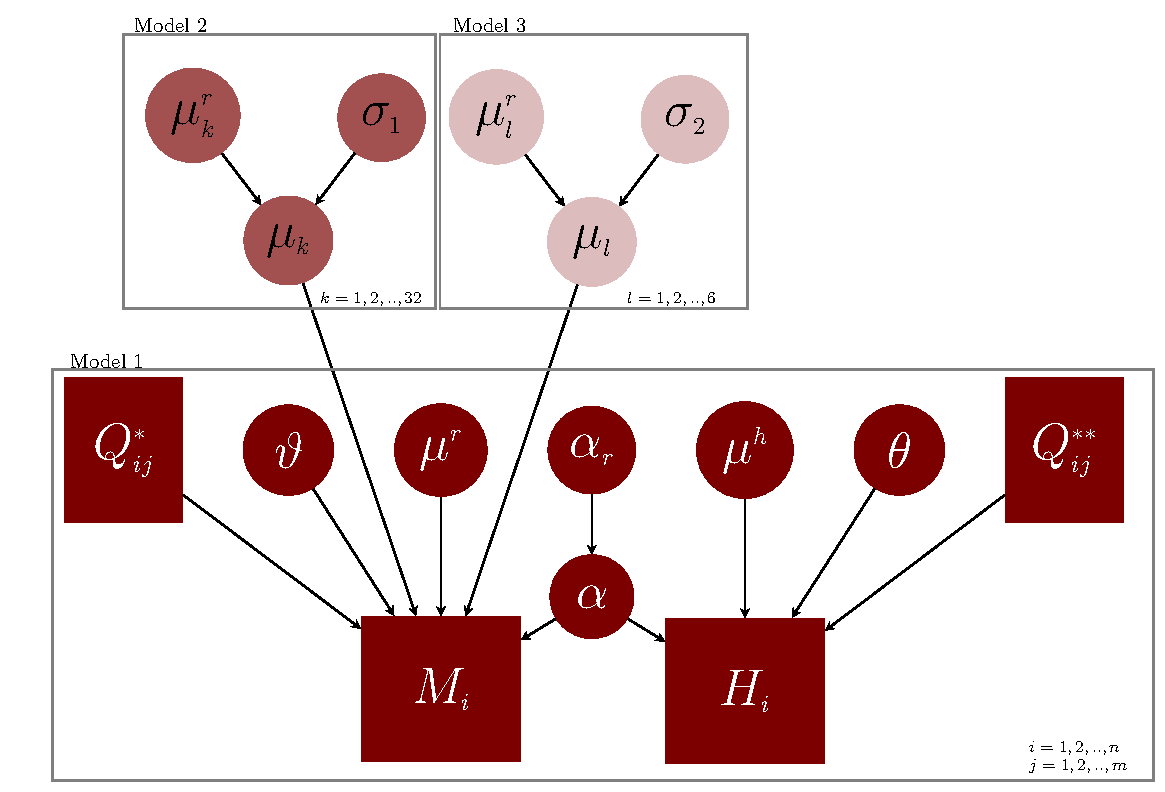
\includegraphics[width=350px]{JerModCOVID19_ROJO} \end{center}

\textbf{Figure 1}. Graphical representation of the model: directed
acyclic grph (DAG)

\begin{center}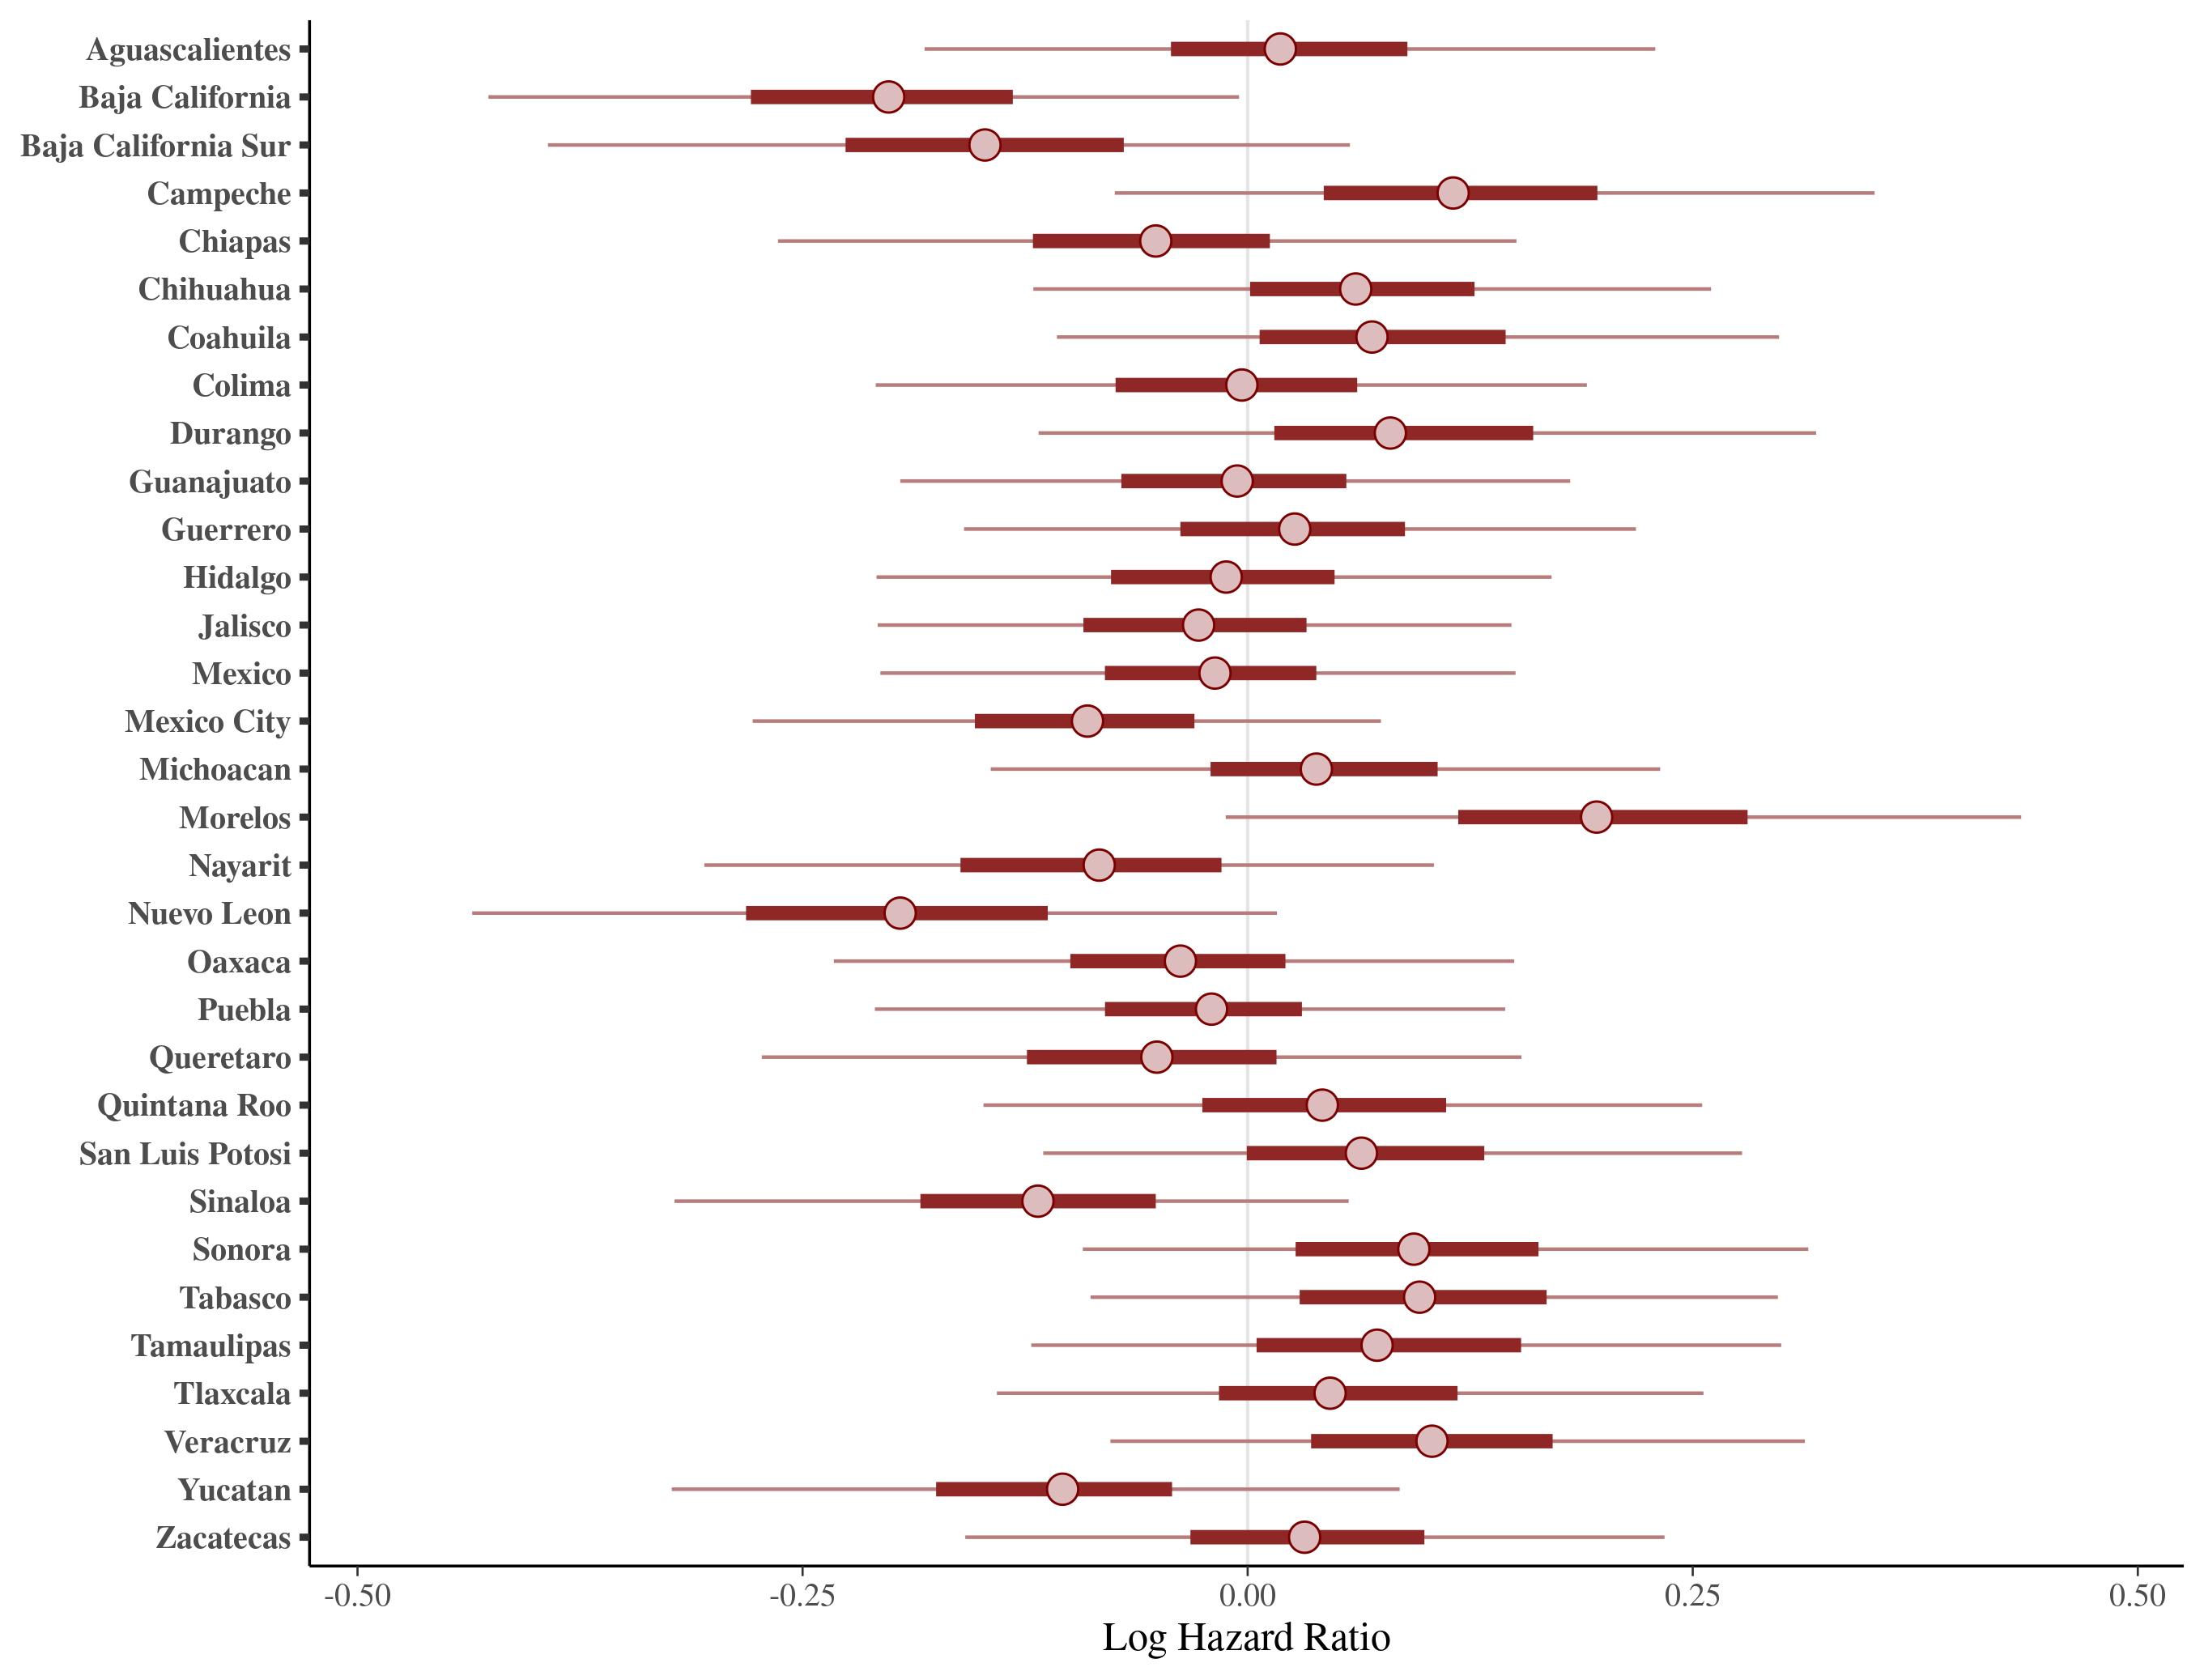
\includegraphics[width=350px]{mu_l_intervalsjer2modi} \end{center}

\textbf{Figure 2}. Log hazard rate for state random effect (95\%
Credible Interval)

\begin{center}
\includegraphics[width=350px]{ppc_plot_modi_mort} \end{center}

\textbf{Figure 3}. Posterior predictive distribution density plot for
deaths

\begin{center}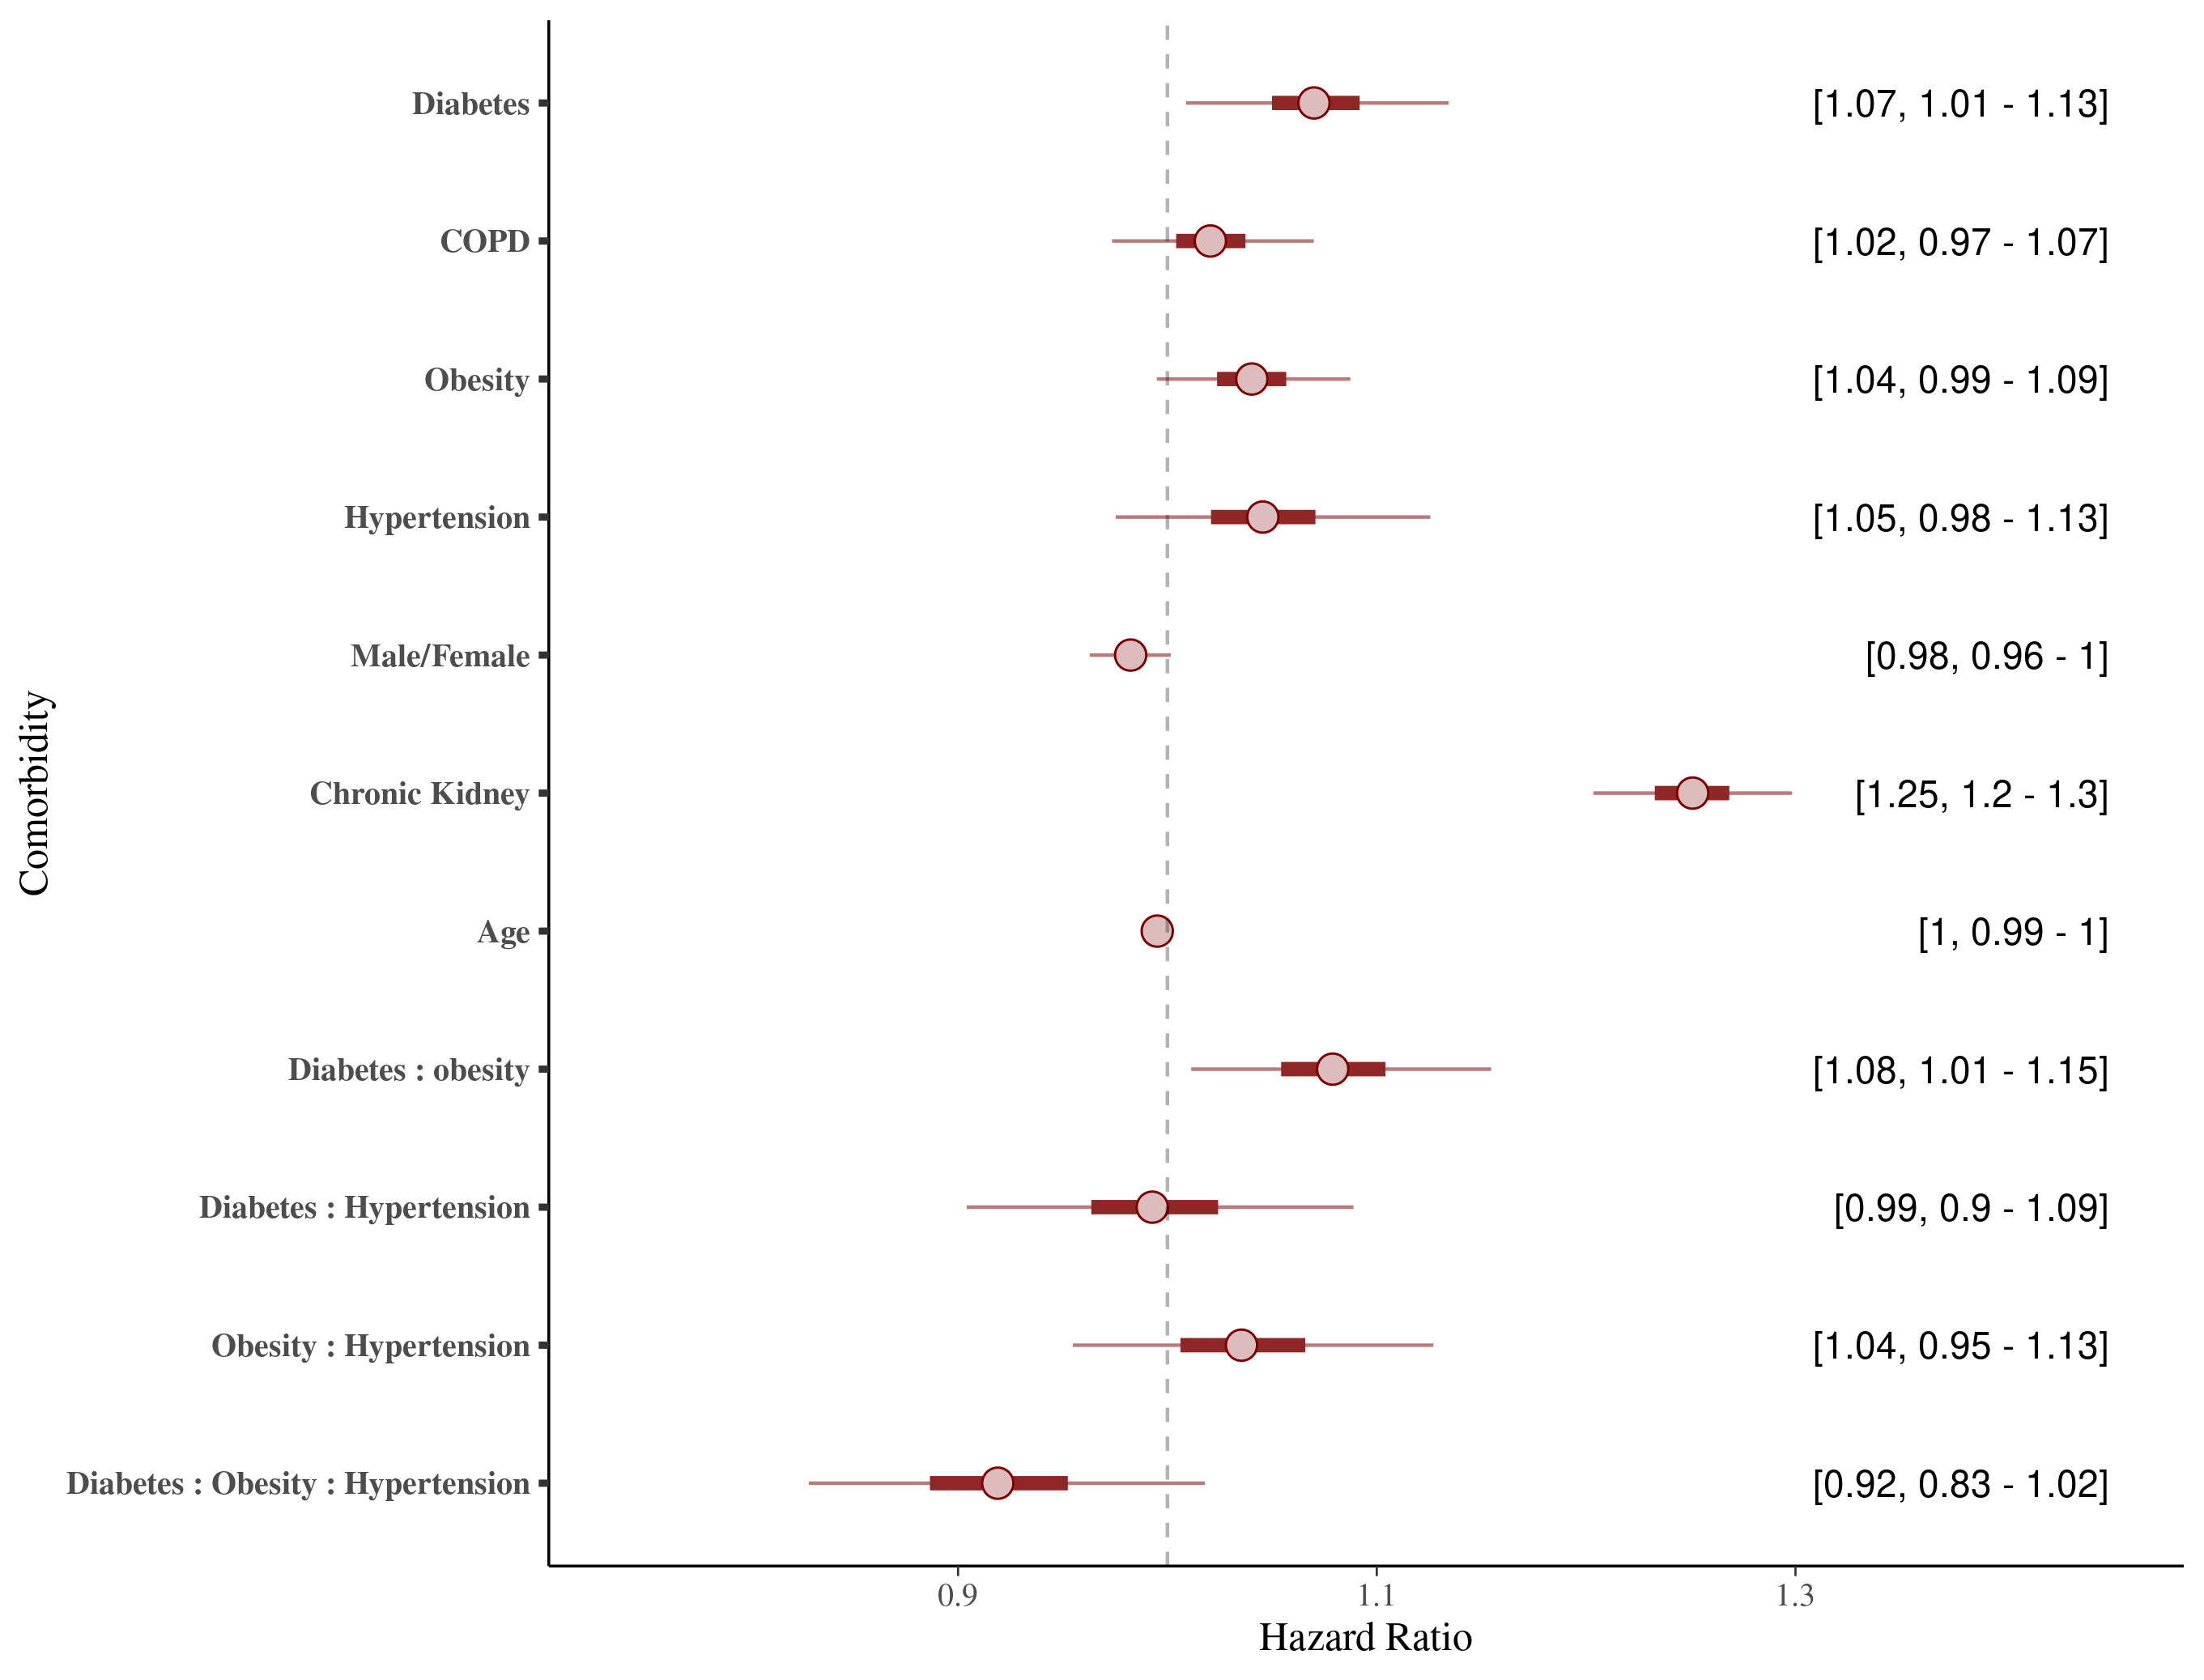
\includegraphics[width=350px]{beta_intervalsjer2modi} \end{center}

\textbf{Figure 4}. Effect on time from hospitalization to death by
covariates included in the final model.

\begin{Shaded}
\begin{Highlighting}[]
\CommentTok{#table_Comorbidites = read.csv("../ArtículoAbril2021/tableOne_comorbidities&Times.csv",row.names= 1)}
\NormalTok{table_Comorbidities =}\StringTok{ }\KeywordTok{read.csv}\NormalTok{(}\StringTok{"../ArtículoAbril2021/tableOne_comorbidities&Times.csv"}\NormalTok{,}\DataTypeTok{row.names=} \DecValTok{1}\NormalTok{)}
\CommentTok{# tibble::print.tbl_df(table)}
\NormalTok{knitr}\OperatorTok{::}\KeywordTok{kable}\NormalTok{(table_Comorbidities,}
             \CommentTok{#row.names = T, }
             \DataTypeTok{caption =} \StringTok{"Comorbidites"}\NormalTok{)}
\end{Highlighting}
\end{Shaded}

\begin{longtable}[]{@{}lllllllr@{}}
\caption{Comorbidites}\tabularnewline
\toprule
\begin{minipage}[b]{0.20\columnwidth}\raggedright
\strut
\end{minipage} & \begin{minipage}[b]{0.09\columnwidth}\raggedright
State.managed\strut
\end{minipage} & \begin{minipage}[b]{0.08\columnwidth}\raggedright
IMSS\strut
\end{minipage} & \begin{minipage}[b]{0.08\columnwidth}\raggedright
ISSSTE\strut
\end{minipage} & \begin{minipage}[b]{0.11\columnwidth}\raggedright
Private.healthcare.provider\strut
\end{minipage} & \begin{minipage}[b]{0.09\columnwidth}\raggedright
SEDENA.SEMAR.PEMEX\strut
\end{minipage} & \begin{minipage}[b]{0.08\columnwidth}\raggedright
SSA\strut
\end{minipage} & \begin{minipage}[b]{0.05\columnwidth}\raggedleft
Missing.data\strut
\end{minipage}\tabularnewline
\midrule
\endfirsthead
\toprule
\begin{minipage}[b]{0.20\columnwidth}\raggedright
\strut
\end{minipage} & \begin{minipage}[b]{0.09\columnwidth}\raggedright
State.managed\strut
\end{minipage} & \begin{minipage}[b]{0.08\columnwidth}\raggedright
IMSS\strut
\end{minipage} & \begin{minipage}[b]{0.08\columnwidth}\raggedright
ISSSTE\strut
\end{minipage} & \begin{minipage}[b]{0.11\columnwidth}\raggedright
Private.healthcare.provider\strut
\end{minipage} & \begin{minipage}[b]{0.09\columnwidth}\raggedright
SEDENA.SEMAR.PEMEX\strut
\end{minipage} & \begin{minipage}[b]{0.08\columnwidth}\raggedright
SSA\strut
\end{minipage} & \begin{minipage}[b]{0.05\columnwidth}\raggedleft
Missing.data\strut
\end{minipage}\tabularnewline
\midrule
\endhead
\begin{minipage}[t]{0.20\columnwidth}\raggedright
n\strut
\end{minipage} & \begin{minipage}[t]{0.09\columnwidth}\raggedright
8,462\strut
\end{minipage} & \begin{minipage}[t]{0.08\columnwidth}\raggedright
237,913\strut
\end{minipage} & \begin{minipage}[t]{0.08\columnwidth}\raggedright
37,652\strut
\end{minipage} & \begin{minipage}[t]{0.11\columnwidth}\raggedright
17,121\strut
\end{minipage} & \begin{minipage}[t]{0.09\columnwidth}\raggedright
20,580\strut
\end{minipage} & \begin{minipage}[t]{0.08\columnwidth}\raggedright
139,164\strut
\end{minipage} & \begin{minipage}[t]{0.05\columnwidth}\raggedleft
NA\strut
\end{minipage}\tabularnewline
\begin{minipage}[t]{0.20\columnwidth}\raggedright
Time from symptoms to hospitalization (median {[}IQR{]})\strut
\end{minipage} & \begin{minipage}[t]{0.09\columnwidth}\raggedright
3.10 {[}2.10, 7.10{]}\strut
\end{minipage} & \begin{minipage}[t]{0.08\columnwidth}\raggedright
5.10 {[}2.10, 8.10{]}\strut
\end{minipage} & \begin{minipage}[t]{0.08\columnwidth}\raggedright
5.10 {[}3.10, 7.10{]}\strut
\end{minipage} & \begin{minipage}[t]{0.11\columnwidth}\raggedright
6.10 {[}3.10, 9.10{]}\strut
\end{minipage} & \begin{minipage}[t]{0.09\columnwidth}\raggedright
4.10 {[}2.10, 7.10{]}\strut
\end{minipage} & \begin{minipage}[t]{0.08\columnwidth}\raggedright
5.10 {[}3.10, 7.10{]}\strut
\end{minipage} & \begin{minipage}[t]{0.05\columnwidth}\raggedleft
0.0\strut
\end{minipage}\tabularnewline
\begin{minipage}[t]{0.20\columnwidth}\raggedright
Time from hospitalization to death (median {[}IQR{]})\strut
\end{minipage} & \begin{minipage}[t]{0.09\columnwidth}\raggedright
154.10 {[}12.10, 316.10{]}\strut
\end{minipage} & \begin{minipage}[t]{0.08\columnwidth}\raggedright
21.10 {[}6.10, 214.10{]}\strut
\end{minipage} & \begin{minipage}[t]{0.08\columnwidth}\raggedright
107.10 {[}8.10, 267.10{]}\strut
\end{minipage} & \begin{minipage}[t]{0.11\columnwidth}\raggedright
197.10 {[}60.10, 322.10{]}\strut
\end{minipage} & \begin{minipage}[t]{0.09\columnwidth}\raggedright
170.10 {[}17.10, 310.10{]}\strut
\end{minipage} & \begin{minipage}[t]{0.08\columnwidth}\raggedright
120.10 {[}8.10, 288.10{]}\strut
\end{minipage} & \begin{minipage}[t]{0.05\columnwidth}\raggedleft
0.0\strut
\end{minipage}\tabularnewline
\begin{minipage}[t]{0.20\columnwidth}\raggedright
Diabetes = NO (\%)\strut
\end{minipage} & \begin{minipage}[t]{0.09\columnwidth}\raggedright
5765 (68.3)\strut
\end{minipage} & \begin{minipage}[t]{0.08\columnwidth}\raggedright
159325 (67.0)\strut
\end{minipage} & \begin{minipage}[t]{0.08\columnwidth}\raggedright
23685 (63.5)\strut
\end{minipage} & \begin{minipage}[t]{0.11\columnwidth}\raggedright
12621 (74.8)\strut
\end{minipage} & \begin{minipage}[t]{0.09\columnwidth}\raggedright
14938 (73.0)\strut
\end{minipage} & \begin{minipage}[t]{0.08\columnwidth}\raggedright
94834 (68.6)\strut
\end{minipage} & \begin{minipage}[t]{0.05\columnwidth}\raggedleft
0.4\strut
\end{minipage}\tabularnewline
\begin{minipage}[t]{0.20\columnwidth}\raggedright
COPD = NO (\%)\strut
\end{minipage} & \begin{minipage}[t]{0.09\columnwidth}\raggedright
8218 (97.3)\strut
\end{minipage} & \begin{minipage}[t]{0.08\columnwidth}\raggedright
228676 (96.2)\strut
\end{minipage} & \begin{minipage}[t]{0.08\columnwidth}\raggedright
35914 (96.3)\strut
\end{minipage} & \begin{minipage}[t]{0.11\columnwidth}\raggedright
16521 (97.7)\strut
\end{minipage} & \begin{minipage}[t]{0.09\columnwidth}\raggedright
20052 (98.0)\strut
\end{minipage} & \begin{minipage}[t]{0.08\columnwidth}\raggedright
134050 (96.8)\strut
\end{minipage} & \begin{minipage}[t]{0.05\columnwidth}\raggedleft
0.4\strut
\end{minipage}\tabularnewline
\begin{minipage}[t]{0.20\columnwidth}\raggedright
Obesity = NO (\%)\strut
\end{minipage} & \begin{minipage}[t]{0.09\columnwidth}\raggedright
6698 (79.3)\strut
\end{minipage} & \begin{minipage}[t]{0.08\columnwidth}\raggedright
190904 (80.3)\strut
\end{minipage} & \begin{minipage}[t]{0.08\columnwidth}\raggedright
30346 (81.3)\strut
\end{minipage} & \begin{minipage}[t]{0.11\columnwidth}\raggedright
14034 (83.0)\strut
\end{minipage} & \begin{minipage}[t]{0.09\columnwidth}\raggedright
15120 (73.8)\strut
\end{minipage} & \begin{minipage}[t]{0.08\columnwidth}\raggedright
105608 (76.3)\strut
\end{minipage} & \begin{minipage}[t]{0.05\columnwidth}\raggedleft
0.3\strut
\end{minipage}\tabularnewline
\begin{minipage}[t]{0.20\columnwidth}\raggedright
Hypertension = NO (\%)\strut
\end{minipage} & \begin{minipage}[t]{0.09\columnwidth}\raggedright
5354 (63.4)\strut
\end{minipage} & \begin{minipage}[t]{0.08\columnwidth}\raggedright
140079 (58.9)\strut
\end{minipage} & \begin{minipage}[t]{0.08\columnwidth}\raggedright
21399 (57.4)\strut
\end{minipage} & \begin{minipage}[t]{0.11\columnwidth}\raggedright
11497 (68.1)\strut
\end{minipage} & \begin{minipage}[t]{0.09\columnwidth}\raggedright
14119 (69.0)\strut
\end{minipage} & \begin{minipage}[t]{0.08\columnwidth}\raggedright
91925 (66.4)\strut
\end{minipage} & \begin{minipage}[t]{0.05\columnwidth}\raggedleft
0.4\strut
\end{minipage}\tabularnewline
\begin{minipage}[t]{0.20\columnwidth}\raggedright
Female = NO (\%)\strut
\end{minipage} & \begin{minipage}[t]{0.09\columnwidth}\raggedright
5005 (59.1)\strut
\end{minipage} & \begin{minipage}[t]{0.08\columnwidth}\raggedright
140865 (59.2)\strut
\end{minipage} & \begin{minipage}[t]{0.08\columnwidth}\raggedright
21729 (57.7)\strut
\end{minipage} & \begin{minipage}[t]{0.11\columnwidth}\raggedright
11385 (66.5)\strut
\end{minipage} & \begin{minipage}[t]{0.09\columnwidth}\raggedright
12707 (61.7)\strut
\end{minipage} & \begin{minipage}[t]{0.08\columnwidth}\raggedright
82163 (59.0)\strut
\end{minipage} & \begin{minipage}[t]{0.05\columnwidth}\raggedleft
0.0\strut
\end{minipage}\tabularnewline
\begin{minipage}[t]{0.20\columnwidth}\raggedright
Chronic Kidney = NO (\%)\strut
\end{minipage} & \begin{minipage}[t]{0.09\columnwidth}\raggedright
8040 (95.2)\strut
\end{minipage} & \begin{minipage}[t]{0.08\columnwidth}\raggedright
222392 (93.6)\strut
\end{minipage} & \begin{minipage}[t]{0.08\columnwidth}\raggedright
35073 (94.0)\strut
\end{minipage} & \begin{minipage}[t]{0.11\columnwidth}\raggedright
16336 (96.7)\strut
\end{minipage} & \begin{minipage}[t]{0.09\columnwidth}\raggedright
19899 (97.2)\strut
\end{minipage} & \begin{minipage}[t]{0.08\columnwidth}\raggedright
133700 (96.6)\strut
\end{minipage} & \begin{minipage}[t]{0.05\columnwidth}\raggedleft
0.4\strut
\end{minipage}\tabularnewline
\begin{minipage}[t]{0.20\columnwidth}\raggedright
Age = NO (\%)\strut
\end{minipage} & \begin{minipage}[t]{0.09\columnwidth}\raggedright
57.00 {[}46.00, 68.00{]}\strut
\end{minipage} & \begin{minipage}[t]{0.08\columnwidth}\raggedright
60.00 {[}49.00, 70.00{]}\strut
\end{minipage} & \begin{minipage}[t]{0.08\columnwidth}\raggedright
62.00 {[}51.00, 72.00{]}\strut
\end{minipage} & \begin{minipage}[t]{0.11\columnwidth}\raggedright
56.00 {[}45.00, 68.00{]}\strut
\end{minipage} & \begin{minipage}[t]{0.09\columnwidth}\raggedright
59.00 {[}47.00, 70.00{]}\strut
\end{minipage} & \begin{minipage}[t]{0.08\columnwidth}\raggedright
57.00 {[}45.00, 67.00{]}\strut
\end{minipage} & \begin{minipage}[t]{0.05\columnwidth}\raggedleft
0.1\strut
\end{minipage}\tabularnewline
\begin{minipage}[t]{0.20\columnwidth}\raggedright
Asthma = NO (\%)\strut
\end{minipage} & \begin{minipage}[t]{0.09\columnwidth}\raggedright
8268 (97.9)\strut
\end{minipage} & \begin{minipage}[t]{0.08\columnwidth}\raggedright
233016 (98.1)\strut
\end{minipage} & \begin{minipage}[t]{0.08\columnwidth}\raggedright
36561 (97.9)\strut
\end{minipage} & \begin{minipage}[t]{0.11\columnwidth}\raggedright
16593 (98.2)\strut
\end{minipage} & \begin{minipage}[t]{0.09\columnwidth}\raggedright
20128 (98.3)\strut
\end{minipage} & \begin{minipage}[t]{0.08\columnwidth}\raggedright
135523 (97.9)\strut
\end{minipage} & \begin{minipage}[t]{0.05\columnwidth}\raggedleft
0.4\strut
\end{minipage}\tabularnewline
\begin{minipage}[t]{0.20\columnwidth}\raggedright
Immunosuppression = NO (\%)\strut
\end{minipage} & \begin{minipage}[t]{0.09\columnwidth}\raggedright
8280 (98.1)\strut
\end{minipage} & \begin{minipage}[t]{0.08\columnwidth}\raggedright
232306 (97.8)\strut
\end{minipage} & \begin{minipage}[t]{0.08\columnwidth}\raggedright
36541 (98.0)\strut
\end{minipage} & \begin{minipage}[t]{0.11\columnwidth}\raggedright
16543 (97.9)\strut
\end{minipage} & \begin{minipage}[t]{0.09\columnwidth}\raggedright
20223 (98.8)\strut
\end{minipage} & \begin{minipage}[t]{0.08\columnwidth}\raggedright
135858 (98.1)\strut
\end{minipage} & \begin{minipage}[t]{0.05\columnwidth}\raggedleft
0.4\strut
\end{minipage}\tabularnewline
\bottomrule
\end{longtable}

\nolinenumbers


\end{document}

